\chapter{Evaluation}

In this chapter, we compare various classifiers for each document representation and discuss the choice of hyperparameters.

For both \textit{BOW} and \textit{doc2vec} document representation, we first show the performance for each classifier individually. The classifier is trained on three lengths of documents -- $200$, $800$ and $3200$ characters. The goal is to see how much better (if at all) is the score for longer documents. At the end of both BOW and doc2vec sections we compare all classifiers for that representation. Finally, we compare both representation and created a combined model using both approaches.


\subsection{Evaluation metric}
As the classes are not balanced (there are $35618$ documents in \textit{children literature} class and only $927$ in \textit{philosophy and ethics}), we will not optimize accuracy but \textit{F1-macro} score, which is defined as:
$$ F_1 = \frac{2PR}{P+R}$$
where $P$ and $R$ are precision and recall averaged over all classes $C_i \in C$ with equal weight\footnote{Which means a misclassification in smaller classes changes the score more than a misclassification in bigger ones.}.

$$P = \frac{1}{|C|}\sum_{i=1}^{|C|}P_i$$
$$R = \frac{1}{|C|}\sum_{i=1}^{|C|}R_i$$

$P_i$ and $R_i$ are then standard precision and recall defined for single class $i$:
$$P_i = \frac{TP_i}{TP_i + FP_i}$$
$$R_i = \frac{TP_i}{TP_i + FN_i}$$

where $TP_i$, $FP_i$ and $FN_i$ are number of true positive, false positive and false negative prediction for class $i$.

\textit{Precision} describes how often was the classifier right when predicting class $i$. \textit{Recall}, on the other hand, captures how often did the classifier predicted class $i$ for documents of class $i$.

To illustrate the computation of the F1-score with \textit{macro} weighting, we compute the test set score for a baseline class predictor which blindly predicts the majority class for every document:
\begin{itemize}
	\item $33771$ documents in the test set
	\item $14$ genres in total
	\item the majority class is \textit{children literature} with $5314$ occurrences
\end{itemize}

For all genres $g$ except for \textit{children literature}, the true positive rate $TP_g$ is equal to $0$ as the predictor never classifies a document in that class. That means that precision $P$ and recall $R$ for those classes is $0$.

For \textit{children literature} class the precision and recall are

\begin{equation}
	\begin{split}
		P_{children\ literature} & = \frac{5314}{33771} = 0.1574 \\
		R_{children\ literature} & = \frac{5314}{5314 + 0} = 1
	\end{split}
\end{equation}

\begin{comment}
\begin{align*}
		P_{children\ literature} &= \frac{5314}{33771} & &= 0.1574 \\
		R_{children\ literature} &= \frac{5314}{5314 + 0} & &= 1
\end{align*}
\end{comment}

as there was no children literature document that was misclassified.

With macro weighting, we get overall precision and recall as 
\begin{equation}
	\begin{split}
	P  & = \frac{1}{14}(13 \cdot 0 + 1 \cdot 0.1574)  = 0.0112 \\
	R & = \frac{1}{14}(13 \cdot 0 + 1 \cdot 1)   = 0.0714
	\end{split}
\end{equation}

Finally, the F1-macro score is then
$$ F_{1-macro} =  \frac{2PR}{P+R} = \frac{2 \cdot 0.0112 \cdot 0.0714}{ 0.0112 + 0.0714} = 0.0194$$

The accuracy, on the other hand, would have been $\frac{5314}{33771} = 0.1574$ which is much higher than the F1-score as the metric does not take class sizes into account. To train the classifier to perform well on all $14$ classes, we optimize the F1-score and only report accuracy for comparison.


\section{Bag of Words}
First, we represent the documents as \textit{binary} bag of words and explore how does the vocabulary size influence the classification performance. As the time and space complexity of the model training are dependent on the size of vocabulary, we want to know if the added complexity brings boost in performance or if the models are overfitted on the training vocabulary. The performance is shown for vocabulary sizes from $1000$ words up to $50000$ words.

When limiting the vocabulary size to $n$ words, we select the $n$ most frequent words which appear in less than $50\ \%$ of all documents. These words also have to occur in at least $5$ distinct documents to be considered for the vocabulary at all. For short documents ($200$ characters, only score for vocabulary up to $30000$ words is shown as the performance stays constant for bigger vocabulary sizes. The reason for that is that if we filter out words occurring in less than $5$ documents, there are only ca. $32000$ words left.

In the following, we compare the classification performance of Naive Bayes classifier, Logistic Regression and feed-forward neural network with two hidden layers. 

\subsection{Naive Bayes}
The Naive Bayes classifier turned out to be a very decent model for the short documents where it reached the same result as logistic regression while having training time under 1 second\footnote{Training was done on a single core on a computer with 2.5 GHz Intel Core i7 CPU}. The performance of Naive Bayes classifier improved with increasing the vocabulary size as shown in \cref{fig:naivebayes}. However, the F1-score for short texts improved by less than $0.01$ when increasing the vocabulary size from $20000$ to $30000$. For middle-length texts, the score improved by only $0.001$ when increasing the vocabulary size from $40000$ to $50000$. 



The best F1-score and accuracy for all three document lengths are listed in \cref{tbl:naivebayes}.

\begin{figure}[h]
	\centering
	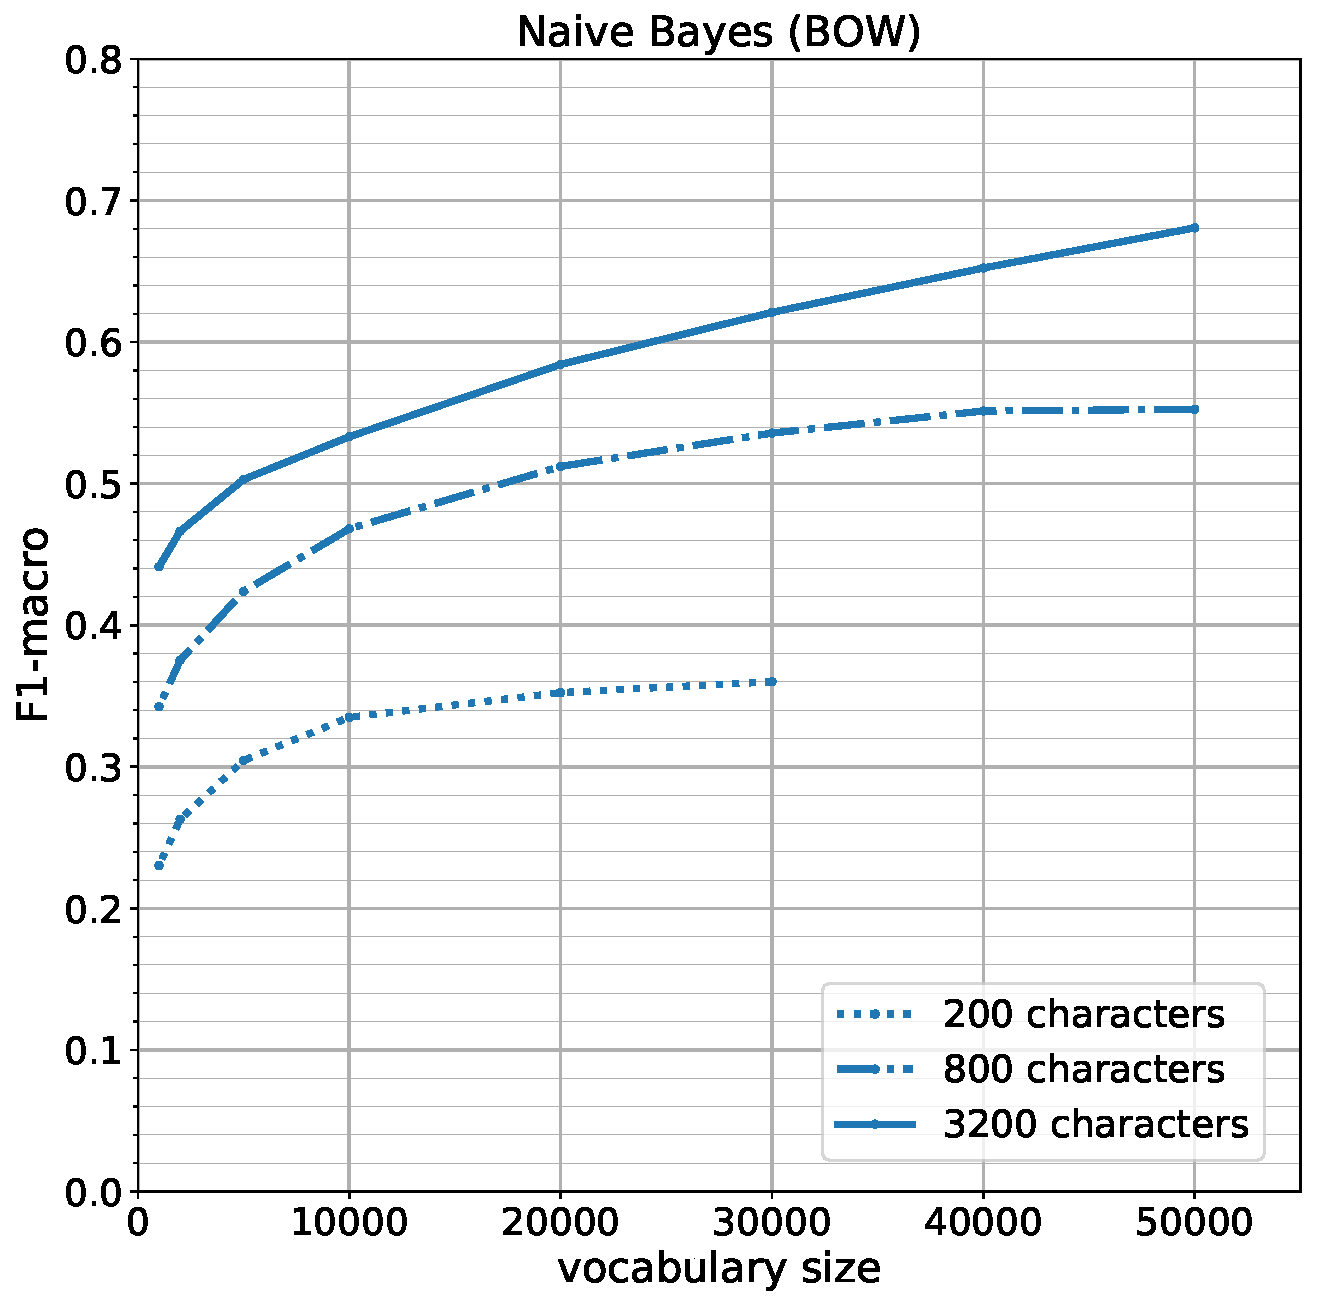
\includegraphics[height=0.3\textheight]{img/05_bow_nb}
	\caption{F1-macro score comparison for Naive Bayes based on text length and vocabulary size.}
	\label{fig:naivebayes}
\end{figure}

\begin{table}[h]
	\centering
	\begin{tabular}{|l|r|r|}\hline
		Document length (vocabulary size) & F1-macro score & Accuracy \\
		\hline
		$200$ chars ($30000$ words)    &   $0.360$      & $0.413$       \\
		$800$ chars ($50000$ words)     &  $0.553$   & $0.572$        \\
		$3200$ chars ($50000$ words)    &  $0.681$   & $0.678$    \\
		\hline
	\end{tabular}
	\caption{Best performance of \textbf{Naive Bayes} on \textbf{binary BOW} for each document length.}
	\label{tbl:naivebayes}
\end{table}


\begin{comment}
For short texts ($200$ characters), classifier reached F1-score $0.396$ and $0.418$ accuracy, for middle-length texts ($800$ characters) $0.571$ F1-score and $0.570$ accuracy. For the long texts of length $3200$ characters, F1-score for Naive Bayes reached $0.615$ and accuracy $0.613$.
\end{comment}

%%%%%%%%%%%%%%%%%%%%%%%%%%%%%%%%%%
%%%%% LOGISTIC REGRESSION %%%%%%%%
%%%%%%%%%%%%%%%%%%%%%%%%%%%%%%%%%%
\subsection{Logistic Regression}
Logistic Regression on binary BOW performed better than Naive Bayes for short and medium-length documents. \cref{fig:bow_logreg} shows the F1-scores for all tested vocabulary sizes and \cref{tbl:bow_logreg} lists best results of the Logistic Regression for each document length.

\begin{figure}[h]
	\centering
	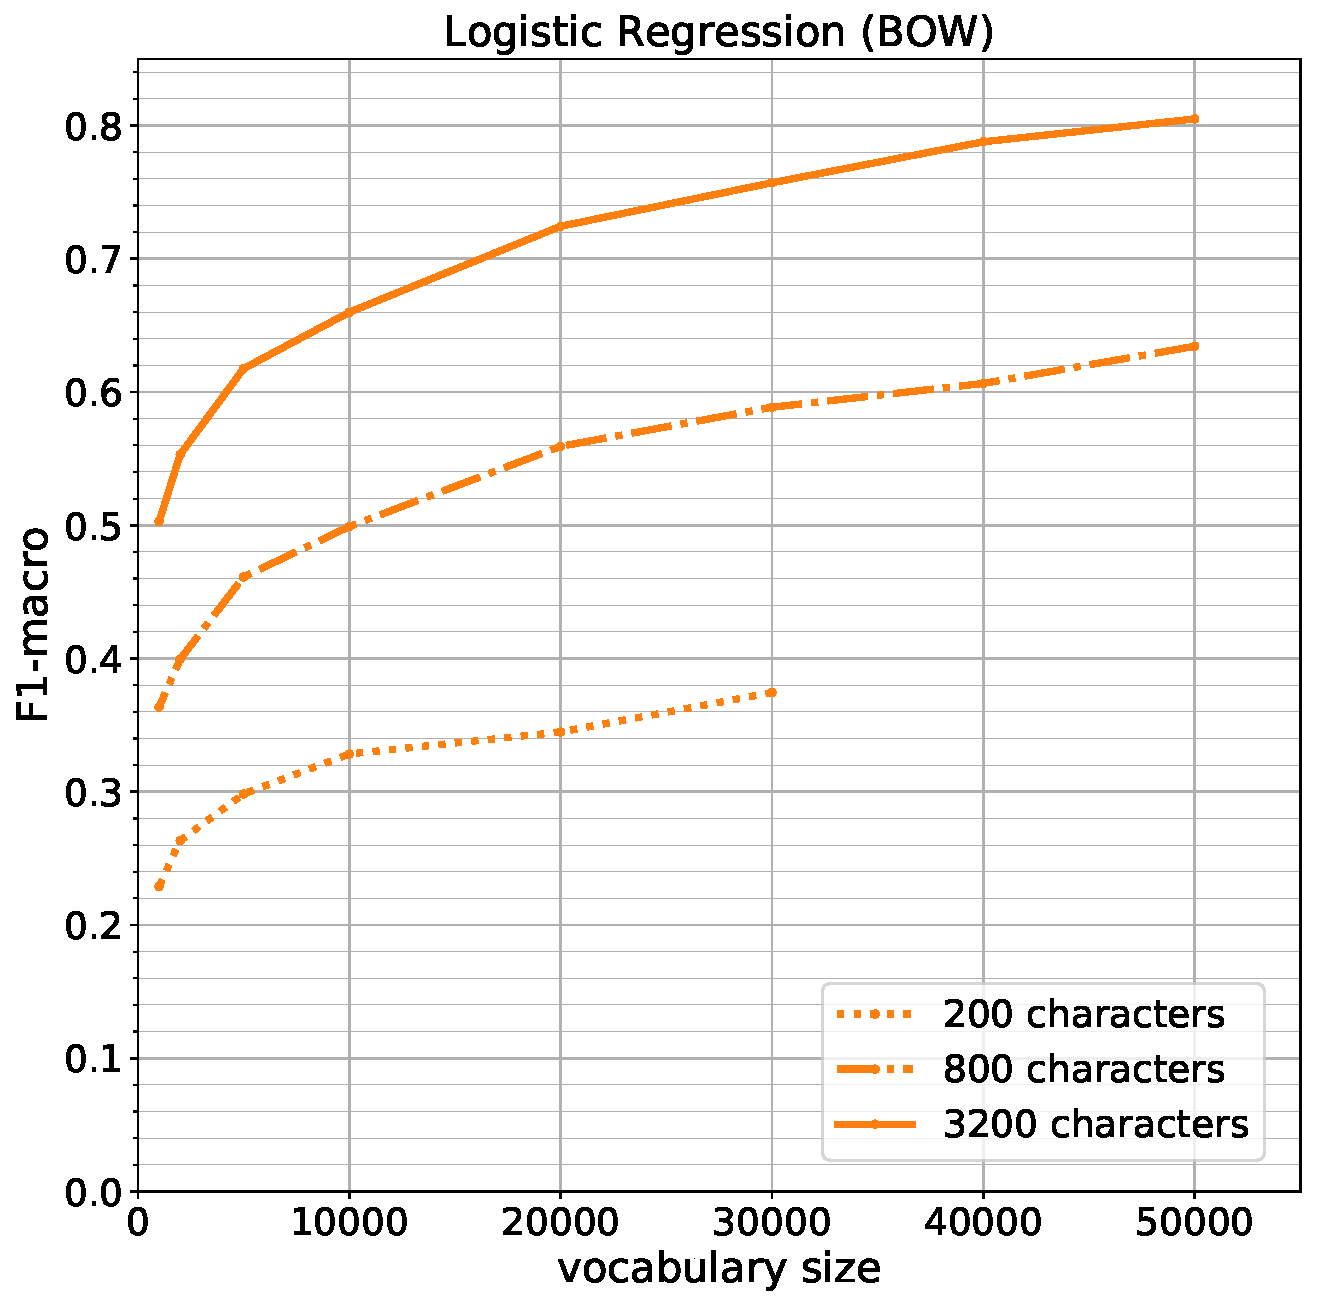
\includegraphics[height=0.3\textheight]{img/05_bow_logreg}
	\caption{F1-macro score comparison for Logistic Regression with binary BOW representation based on text length and vocabulary size.}
	\label{fig:bow_logreg}
\end{figure}

\begin{table}[h]
	\centering
	\begin{tabular}{|l|r|r|}\hline
		Document length (vocabulary size) & F1-macro score & Accuracy \\
		\hline
		$200$ chars ($30000$ words)    &   $0.374$   & $0.398$       \\
		$800$ chars ($50000$ words)     &  $0.634$   & $0.637$        \\
		$3200$ chars ($50000$ words)    &  $0.805$   & $0.802$    \\
		\hline
	\end{tabular}
	\caption{Best performance of \textbf{Logistic Regression} on \textbf{binary BOW} for each document length.}
	\label{tbl:bow_logreg}
\end{table}

For vocabulary size greater than $10000$, training with all $191363$ documents does not fit into $16$ GB of RAM. Therefore, we used \textit{sklearn}'s stochastic gradient descent with logistic loss which corresponds to logistic regression.

The best Logistic Regression classifier on binary BOW trained on long documents with vocabulary containing $50000$ words reached F1-score $0.805$ and accuracy $0.801$.

For each vocabulary size, \textit{grid search} was used to find the best regularization strength parameter $\alpha$. Generally, the optimal $\alpha$ value increased with document size and decreased with the size of vocabulary. The optimal $\alpha$ for the already mentioned best classifier was $0.0003$.


%%%%%%%%%%%%%%%%%%%%%%%%%%%%%%%%%%
%%%%% Feed-forward NN%%%% %%%%%%%%
%%%%%%%%%%%%%%%%%%%%%%%%%%%%%%%%%%
\subsection{Feed-forward NN}
Next classifier we tried out for the binary BOW representation was a simple feed-forward neural network with $2$ hidden layers of $200$ and $100$ neurons. We used \textit{ReLU} as an activation function for hidden layers, and \textit{softmax} on the output layer.

To decrease overfitting of the net, dropout layers were added between the layers with following coefficients:
\begin{itemize}
  \item $\textbf{0.4}$ between input and first hidden layer with $200$ neurons
  \item $\textbf{0.1}$ between first hidden layer with $200$ neurons and second with $100$ neurons
\end{itemize}
\cref{fig:bow_nn_architecture} shows the architecture of the net.

In \cref{fig:bow_nn} we can see that the F1-score of the feed-forward neural network improves with increasing vocabulary size as did the previous two algorithms. Even between the vocabulary size of $40000$ and $50000$, there is still about $0.02$ score difference.

The best F1-score reached for long documents was $0.849$ which is about $4\ \%$ better than the logistic regression. That comes as no surprise as logistic regression is equivalent to neural network with softmax output layer activation and no hidden layer.\footnote{except for regularization} As our net has two hidden layers, it is then computationally stronger than logistic regression. Best results also for shorter documents is shown in \cref{tbl:bow_nn}.

For long documents, the net overfitted massively the training data and reached accuracy score of $99\ \%$ on the training set. One way to deal with the overfit is to increase the dropout rate on the input layer. Another possibility is to decrease the number of neurons in the hidden layer. However, this kind of optimization requires lots of time and computational power and would most likely not bring us more than about $0.5\ \%$ improvement on the score.


\begin{figure}[h]
	\centering
	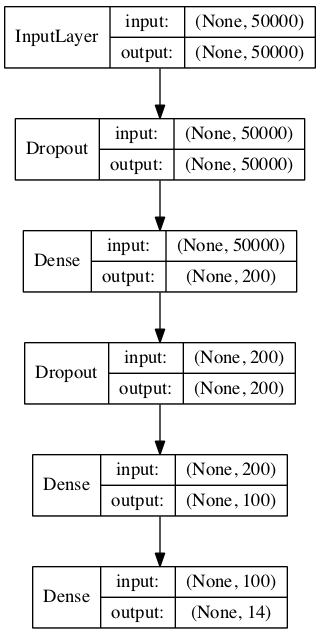
\includegraphics[height=0.3\textheight]{img/bow_nn}
	\caption{Feed-forward NN architecture for $50000$ words in vocabulary}
	\label{fig:bow_nn_architecture}
\end{figure}

\begin{figure}[h]
	\centering
	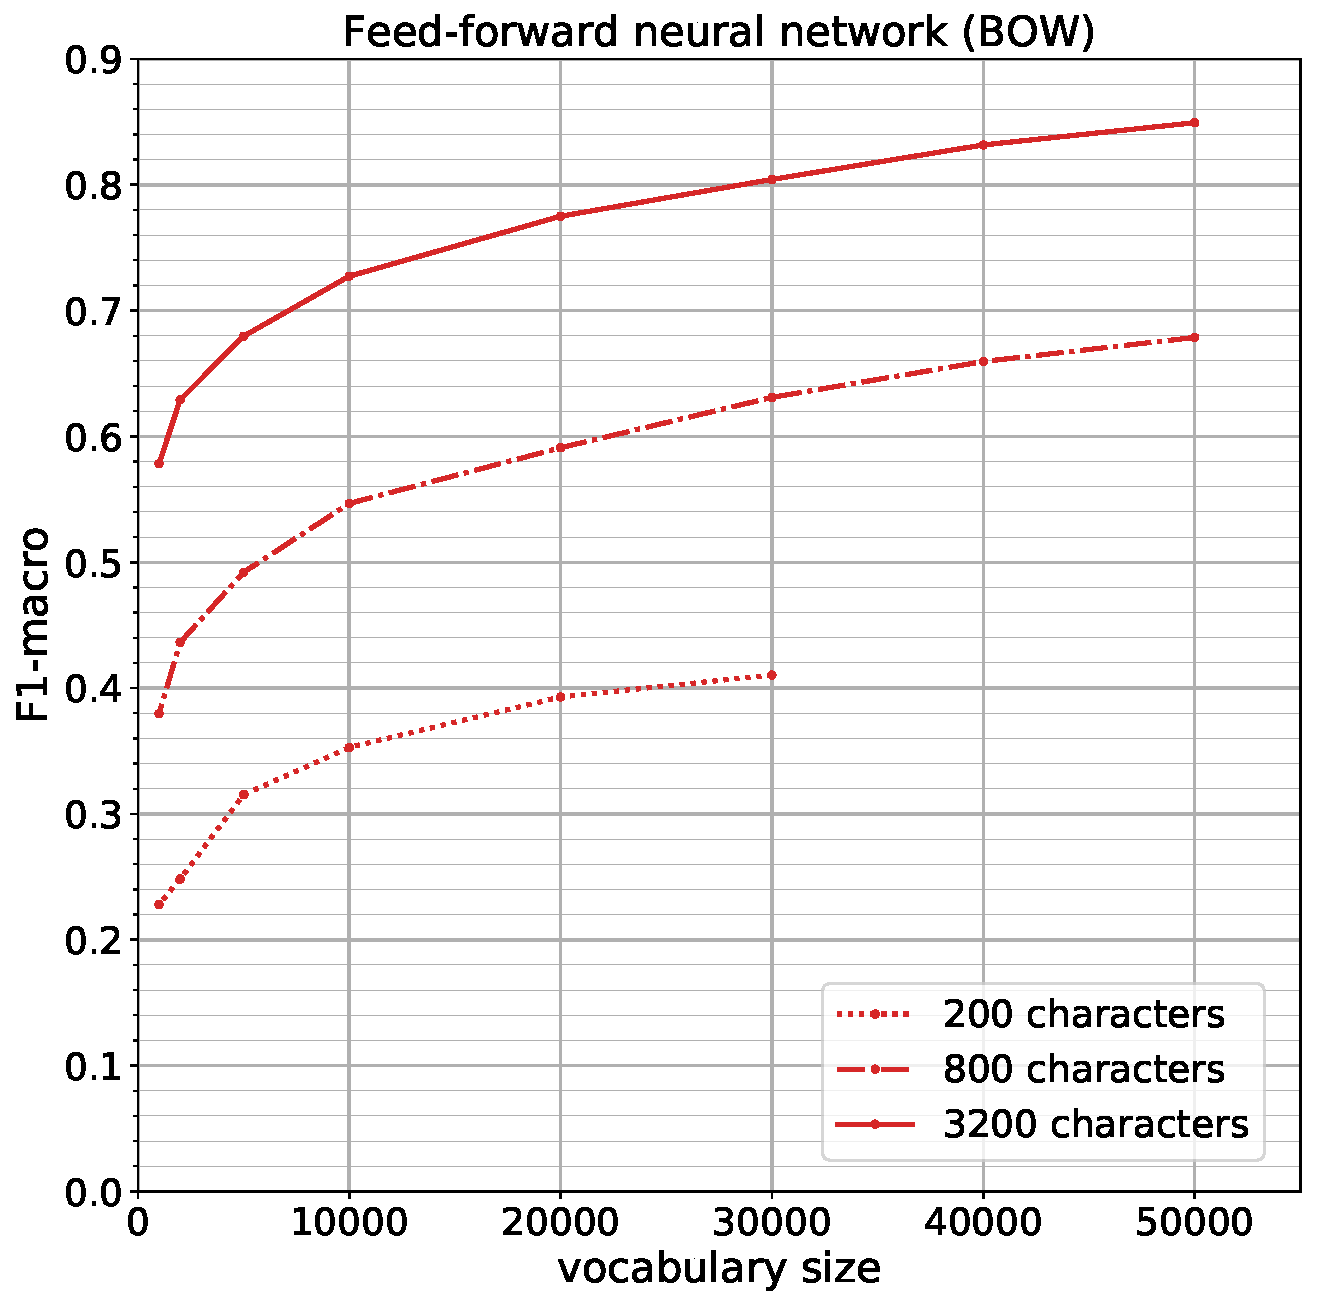
\includegraphics[height=0.3\textheight]{img/05_bow_nn}
	\caption{BOW with feed-forward NN classifier.}
	\label{fig:bow_nn}
\end{figure}


\begin{table}[h]
	\centering
	\begin{tabular}{|l|r|r|}\hline
		Document length (vocabulary size) & F1-macro score & Accuracy \\
		\hline
		$200$ chars  &  $0.410$   & $0.429$   \\
		$800$ chars  &  $0.679$   & $0.680$   \\
		$3200$ chars &  $0.849$   & $0.850$   \\
		\hline
	\end{tabular}
	\caption{Best performance of \textbf{feed-forward NN on binary BOW} for each document length.}
	\label{tbl:bow_nn}
\end{table}

\subsection{Tf-Idf}
Until now, the feature vector for each document was binary. Nevertheless, it performed quite decent. In the following, we represent documents as tf-idf vectors utilizing both the frequency of each word in the given document and the word overall frequency in the training corpus.

To compare with the binary approach, we applied Logistic Regression on top of \textit{Tf-Idf} vectors. Accuracy and F1-scores for all document lengths are shown in \cref{tbl:tfidf}. \cref{fig:05_tfidf} shows that \textit{Tf-Idf} can make use of extra words in the vocabulary as the score for all three document lengths is increasing with the size of vocabulary.

\begin{table}[h]
	\centering
	\begin{tabular}{|l|r|r|}\hline
		Document length (vocabulary size) & F1-macro score & Accuracy \\
		\hline
		$200$ chars  &  $0.395$   & $0.418$   \\
		$800$ chars  &  $0.663$   & $0.664$   \\
		$3200$ chars &  $0.836$   & $0.829$   \\
		\hline
	\end{tabular}
	\caption{Best performance of \textbf{logistic regression} on \textbf{tf-idf} for each document length.}
	\label{tbl:tfidf}
\end{table}

Similarly to the logistic regression on binary BOW, the regularization parameter $\alpha$ decreased with increasing size of vocabulary. The optimal $\alpha$ value for the best models of each document lengths turned at to be the same -- $10 ^{-6}$.

\begin{figure}[h]
	\centering
	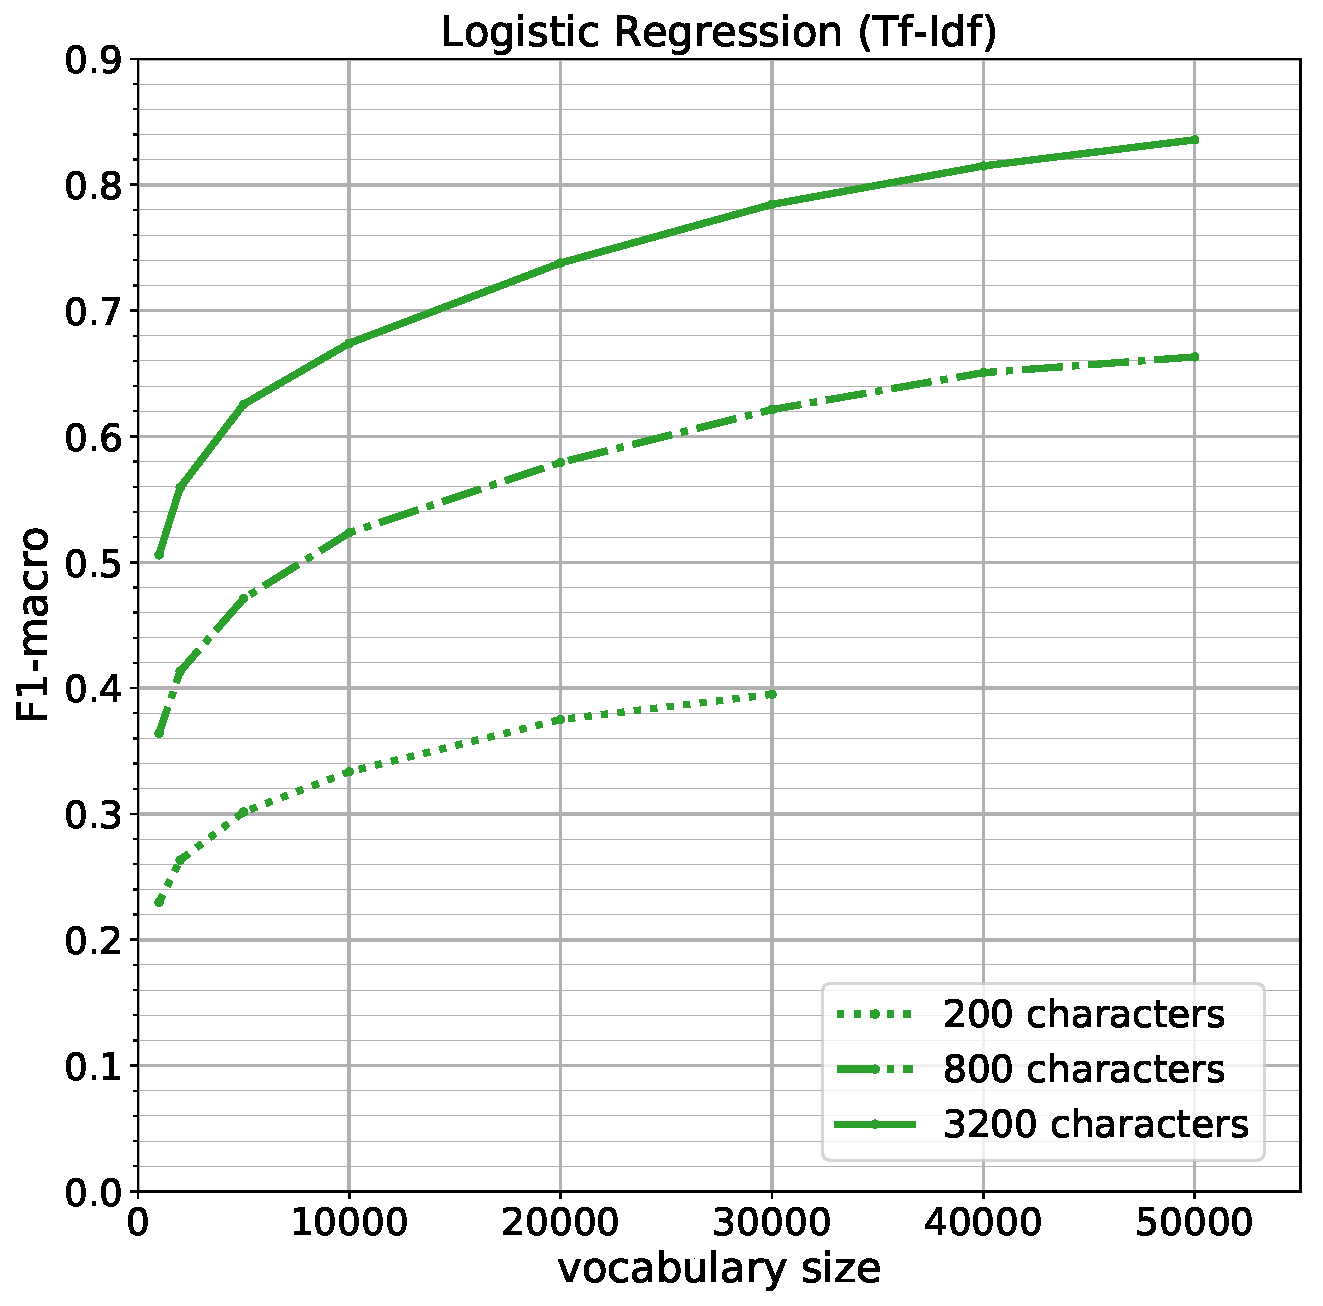
\includegraphics[height=0.3\textheight]{img/05_tfidf}
	\caption{F1-macro score comparison for Logistic Regression on Tf-Idf weighted vectors.}
	\label{fig:05_tfidf}
\end{figure}




\subsection{Summary BOW}

All in all, the score improved with growing vocabulary size for all algorithms and document lengths. For all three document lengths, neural network performed the best out of all algorithms, slightly better than logistic regression on tf-idf. Logistic regression on tf-idf performed better than on binary BOW and the gap increased with growing size of vocabulary. It is probably caused by tf-idf boosting the rare words\footnote{words not in top $10000$ most common words in the corpus} that might be defining the genre.\footnote{For example the word \textit{asteroid} occurred $54$ times in science fiction genre and never in any other genre.}

The Naive Bayes classifier performed the worst out of the tested algorithms. It performed very similar to other algorithms on short documents -- only $0.014$ worse than logistic regression on binary BOW. However, for longer documents, it could not predict genres as good as other algorithms -- falling behind the logistic regression on binary BOW by $0.08$ for middle-length documents and $0.12$ for long documents.

\cref{tbl:bow_comparison} shows the comparison of all algorithms and document lengths. The neural net reached F1-score of $0.849$ and accuracy $0.850$. The logistic regression on tf-idf performed was worse only by $0.013$ which is negligible given a lot higher training complexity and space needed to fit and store the neural net.

\begin{table}[h]
	\centering
	\begin{tabular}{|l|r|r|r|r|}\hline
		Document length & Naive Bayes & Log. reg. & Log. reg. (Tf-Idf) & NN \\
		\hline
		$200$ chars   & $ 0.360$  &  $0.374$  & $0.395$  &  $0.410$   \\
		$800$ chars   & $0.552$  &  $0.634$  & $0.663$  &  $0.679$   \\
		$3200$ chars  & $0.681$  &  $0.805$  & $0.836$  &  $0.849$   \\
		\hline
	\end{tabular}
	\caption{F1-score comparison of classifiers on BOW document representation for each document length.}
	\label{tbl:bow_comparison}
\end{table}


% \subsubsection{Short documents}

For short documents, the training set contained only $30000$ words after low occurrence words were filtered out. To improve the vocabulary quality, we tried out using the vocabulary fitted on the long documents with $3200$ characters expecting it to contain more relevant words and less noise as the vocabulary was fitted on $16$ times more text. However, contrary to our expectations, using this vocabulary actually slightly decreased the performance by about $0.02$ for both $800$ and $200$-character documents. 

The cause for this result is that when vocabulary was choosing top $n$ words based on frequency in the corpus, words with higher frequency in the corpus of long documents were preferred to those with high frequency in the training set of short documents. Therefore, the classification algorithms couldn't utilize the "better vocabulary".

\cref{fig:bow} shows comparisons of all BOW algorithms on each document length.


\begin{figure}
\centering
\begin{subfigure}[t]{.49\textwidth}
	\centering
	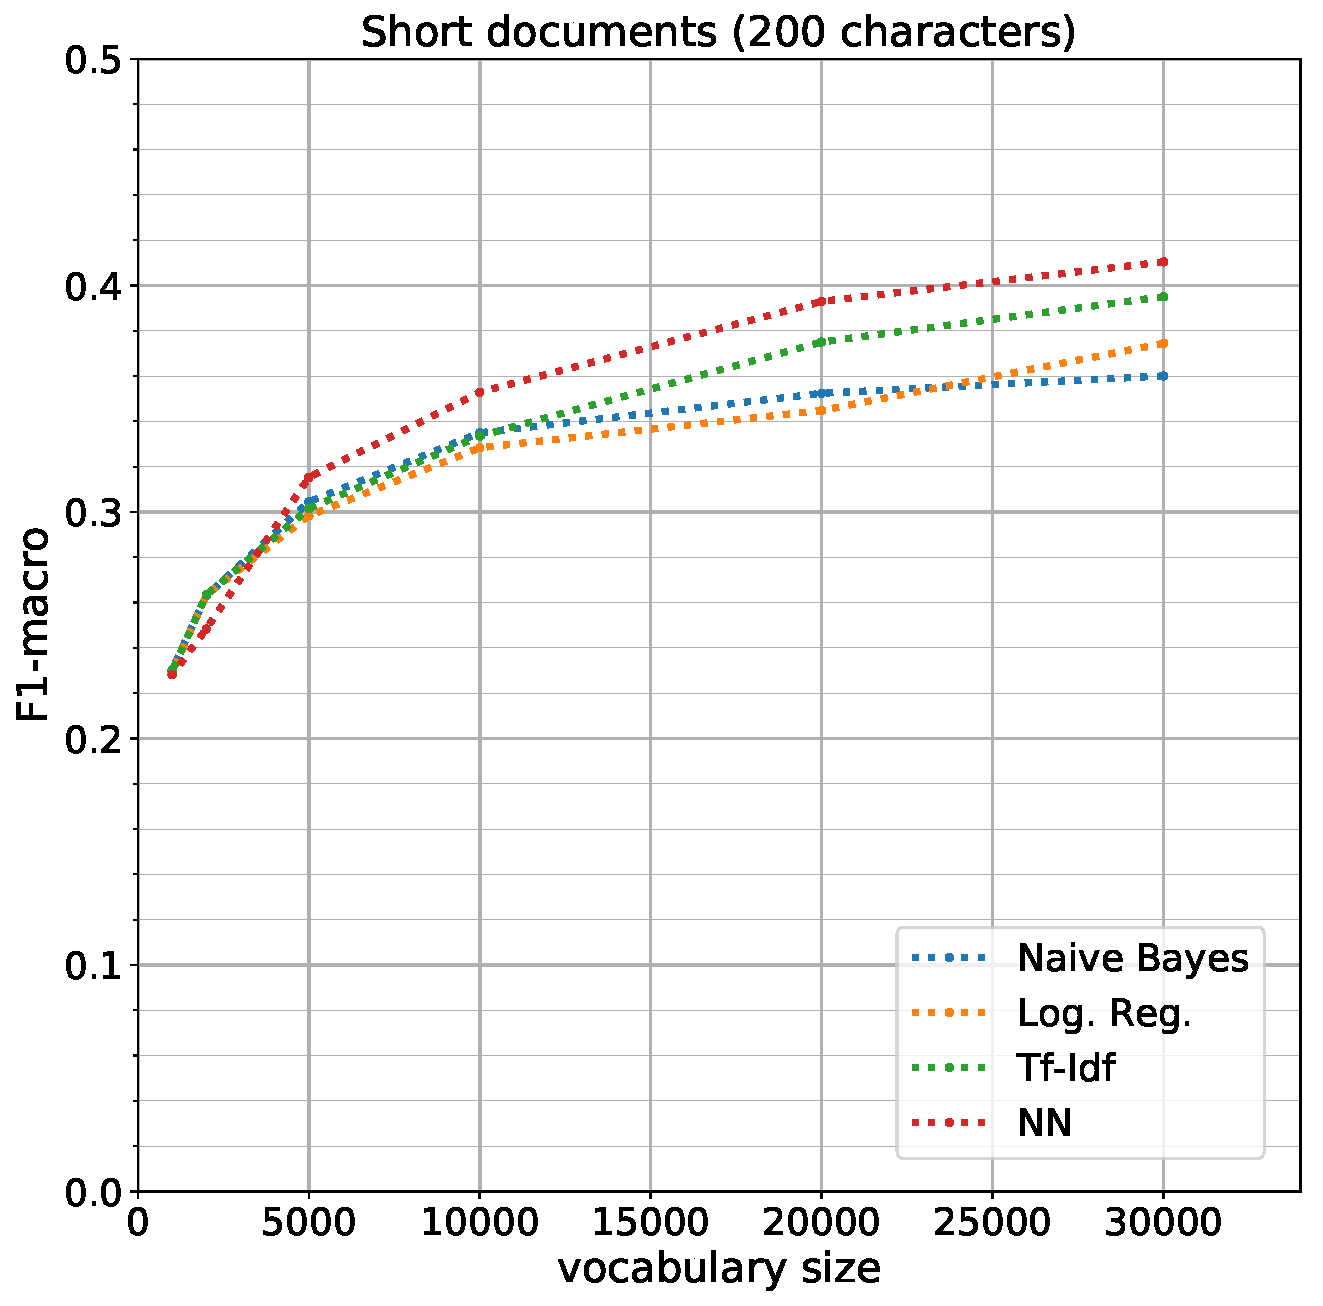
\includegraphics[width=0.99\linewidth]{img/05_bow_200}
	\caption{200 characters}
	\label{fig:05_bow_200}
\end{subfigure}%
\begin{subfigure}[t]{.49\textwidth}
	\centering
	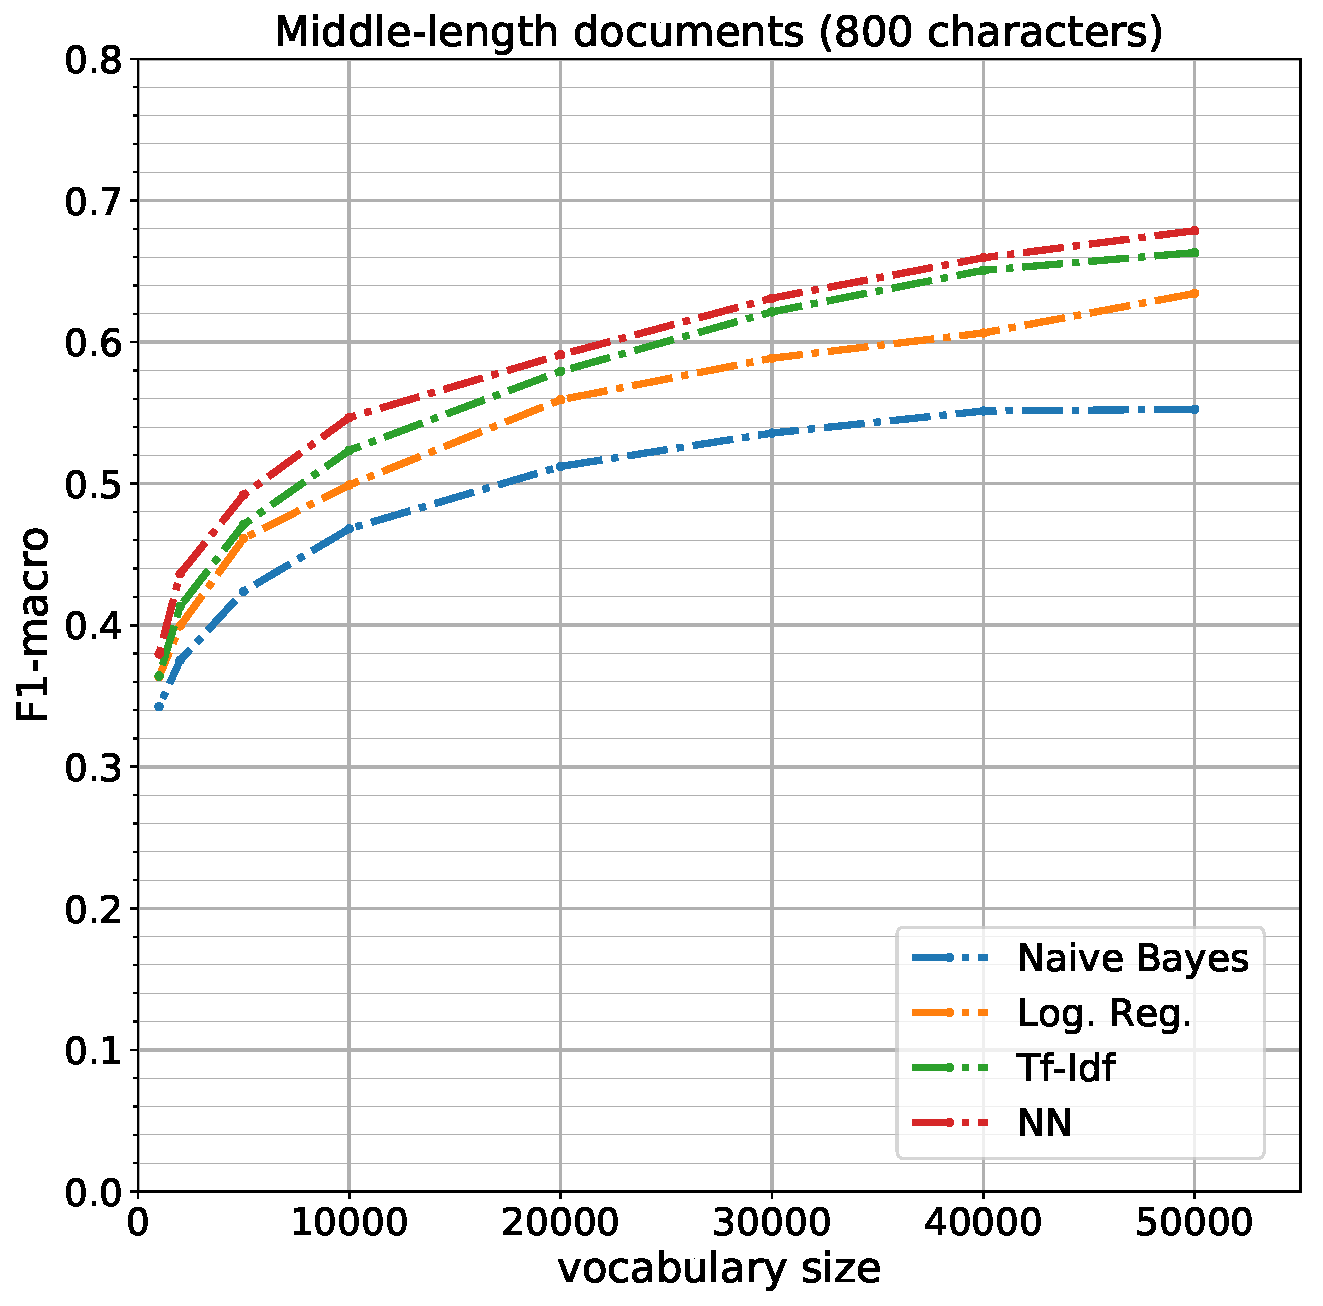
\includegraphics[width=0.99\linewidth]{img/05_bow_800}
	\caption{800 characters}
	\label{fig:05_bow_800}
\end{subfigure}

\begin{subfigure}[t]{.49\textwidth}
	\centering
	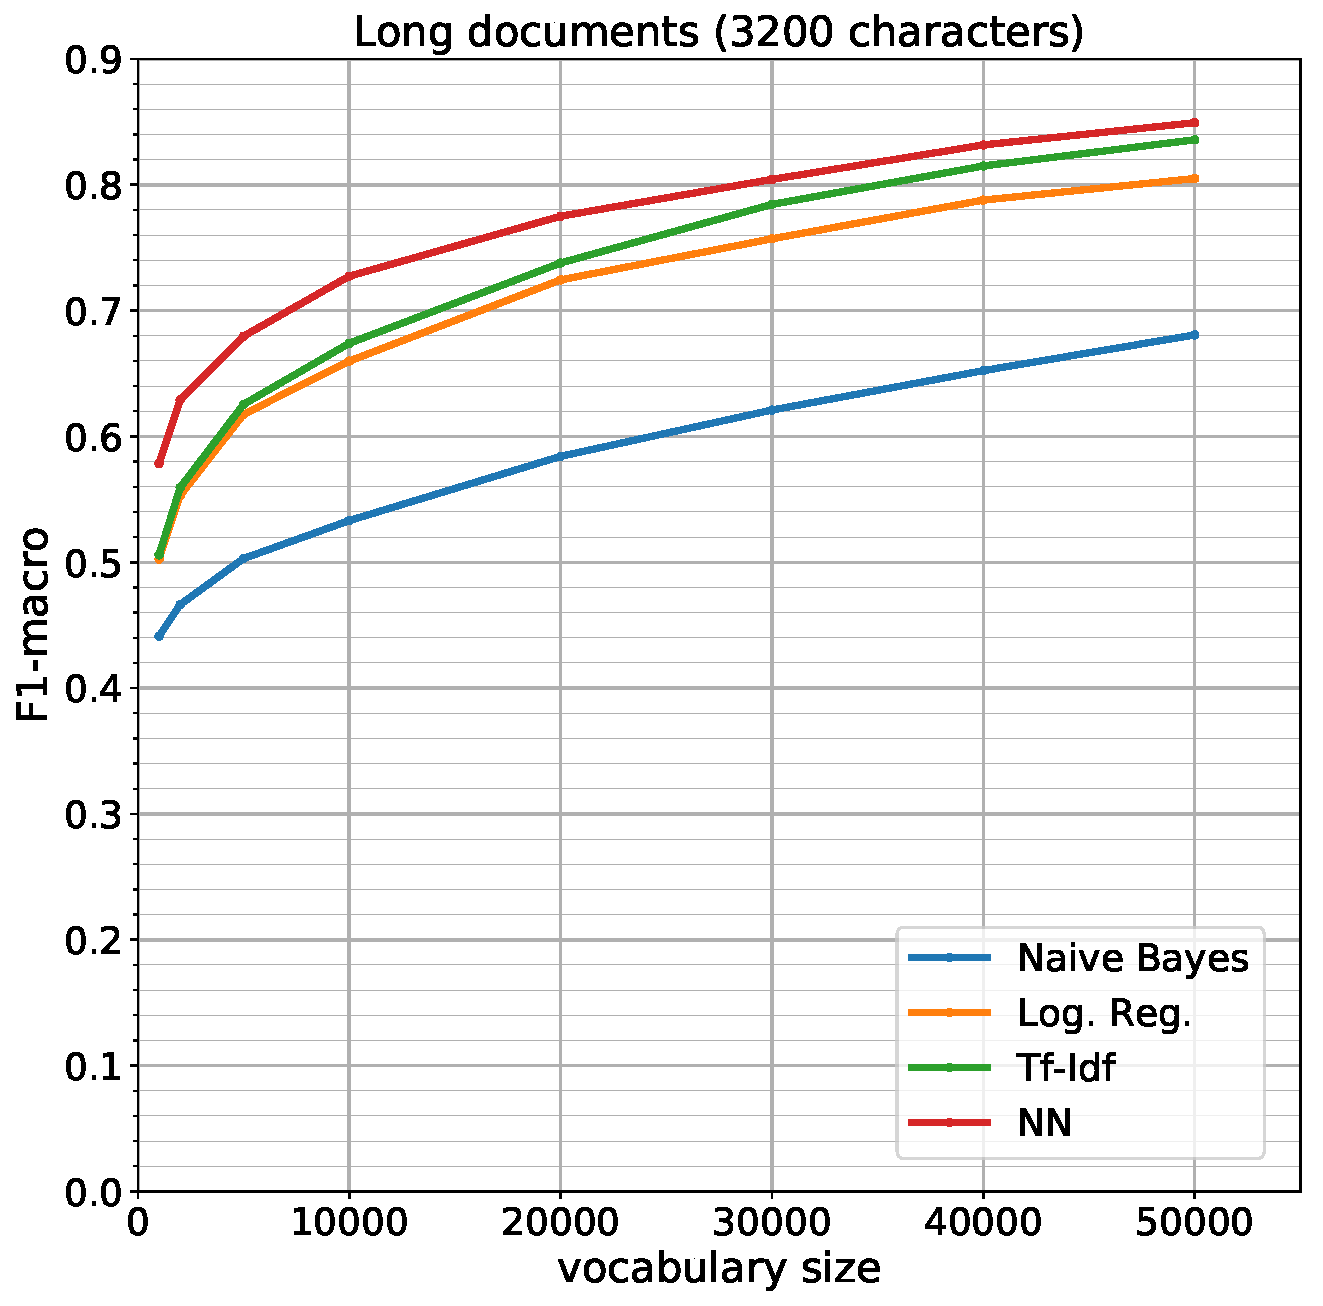
\includegraphics[width=0.99\linewidth]{img/05_bow_3200}
	\caption{3200 characters}
	\label{fig:05_bow_3200}
\end{subfigure}%

\caption{F1-macro score comparison for all BOW algorithms.}
\label{fig:bow}
\end{figure}



\begin{comment}
The reason for this might be that when using vocabulary created on other (even though larger) set, number of words in the shorter texts which are in that vocabulary is lower than when using vocabulary trained directly on documents itself. And fewer words in vocabulary means fewer information about the text (as words not in vocabulary are ignored and skipped), hence worse score.
\end{comment}

%\subsubsection{Medium-length documents}

%\cref{fig:05_bow_800}


%\subsubsection{Long documents}

%\cref{fig:05_bow_3200}



%%%%%%%%%%%%%%%%%%%%%%%%%%%%%%%%%%
%%%%%%%%%%%%%%%%%%%%%%%%%%%%%%%%%%
%%%%%%%%%% DOC2VEC  %%%%%%%%%%%%%%
%%%%%%%%%%%%%%%%%%%%%%%%%%%%%%%%%%
%%%%%%%%%%%%%%%%%%%%%%%%%%%%%%%%%%

\section{Doc2vec}
In the next approach, documents are embedded into a space of several hundred dimensions using \textit{doc2vec}. This representation is a lot smaller and compacter than the previous BOW approach where documents were represented by vectors with up to $50000$ dimensions.

For the document classification, we used similarity metrics to find most similar documents (kNN) or most similar genre vector. Apart from those,  logistic regression and simple neural network with one hidden layer containing $50$ neurons were used.

The training of doc2vec was done using the \textit{gensim}\cite{gensim} module for python and a big hyperparameter search had to be done to make the approach work for our task. The main parameters we had to tune were:

\begin{itemize}
  \item \textit{dimension} of the vectors
  \item choosing between \textit{dbow} and \textit{dm} architecture
  \item \textit{window size}
\end{itemize}

\subsection{Hyperparameter tuning}
For the initial parameter setting, we adopted the parameters from J. H. Lau and T. Baldwin - An Empirical Evaluation of doc2vec with Practical Insights into Document Embedding Generation\cite{doc2vec_params}. They also report improvement when initializing the doc2vec model with word embeddings trained on bigger corpus.

In order to choose the right hyperparameters, we have to find a way to compare trained doc2vec models. As we train not only document vectors but also genre vectors, the quality can be estimated by comparing the inferred documents from the validation set with the genre vectors and computing how often was the vector of the correct genre the most similar one out of all $14$ genre vectors in terms of cosine similarity.

%Models are compared and selected based on "nearest genre classifier".

\subsubsection{Distributed BOW (DBOW) vs. Distributed Memory (DM)}
Le \& Mikolov, the original authors of the Paragraph vector\cite{doc2vec}, 
propose two architectures.

The first one is Distributed Memory where the task is to predict a missing word from the window given the context (surrounding words) and the paragraph vector.

The second architecture is is Distributed bag of words where the net is trained to predict words in a small window given the document vector.

Le \& Mikolov report distributed memory version to perform better.\cite{doc2vec} However, Lau and Baldwin\cite{doc2vec_params} as well as the creators of gensim\cite{gensim} observed the distributed BOW version to obtain better results.

In our experiments, we join the latter as the Distributed BOW version reaches $0.05$ to $0.1$ better score on the task of genre classification than the Distributed Memory architecture.

The following hyperparameter discussion focuses then on the DBOW doc2vec.

\subsubsection{Vector dimension}
Le \& Mikolov used in the original work vectors with $400$ dimensions.\cite{doc2vec}, Lau and Baldwin chose $300$ dimensions.\cite{doc2vec_params}

For our task, number of dimensions between $300$ and $400$ worked the best as well. The performance did not improve for vector sizes bigger than $500$ and for less than $200$ dimensions, the performance started decreasing.

\subsubsection{Window size}
Discuss impact of window size on the quality of vectors for each length.
\subsubsection{Including genre vectors}
\begin{itemize}
	\item way better performance when including genre vectors
	\item tried also to add original book vector (as multiple documents come from the same book) but didn't improve genre prediction
	\item as shown later, it not only improves document embeddings but also enables us to use the nearest genre vector of a text as a decent prediction
\end{itemize}

\subsubsection{Pre-trained word embeddings}
As mentioned before, Lau and Baldwin\cite{doc2vec_params} report improvement when using pre-trained word vectors. For our task, using $GloVe$ vectors with $300$ dimensions trained on Wikipedia improved the score. The improvement was more significant for predictions based on short documents. That comes as no surprise as short documents contain less data to train a good word-embedding than longer documents..

\subsubsection{Learning rate $\alpha$}
The default training rate$ \alpha$ in gensim is $0.025$ which turned out to be too large for our setting. Best working alphas we observed were between $0.0075$ and $0.015$.
\begin{comment}
	And multiplying alpha by 4/5 or 9/10 at the end of every iteration
\end{comment}

\subsubsection{Document shuffling}
Another thing that improves the document vector quality is reshuffling of training samples at the beginning of each epoch. Reshuffling, however considered as a standard for neural net training, is not supported by gensim\footnote{At least not at the time of writing this text -- June 2018} and has to be done manually. Doing so constantly improves the score by couple of percent points.

\subsubsection{Vector inference for new documents}
\begin{itemize}
	\item $3$ infer steps instead of default $5$ in gensim works better
	\item as inferring is not deterministic, nearest genre classifier works best if we infer the vector multiple times (ca 10) and make a majority vote
\end{itemize}

\subsection{Similarity Cosine similarity with genre vectors}

The first classifier we applied after training the doc2vec representation, was \textit{Nearest genre vector}. It simply chooses the nearest genre vector to a document using cosine similarity between the vectors.

\begin{itemize}
	\item show table of performance with/wo genre and book vectors and w/wo GloVe embeddings
	\item $O(1)$ time and space, no training needed
\end{itemize}

Do multiple infers and majority vote - improves ca. $2\ \%$.

3 infer steps instead of 5 - default in gensim

\subsection{K most similar books (KNN)}

KNN - slow, cosine sim. better than eucl.

For $k = 10$, the performance was $.809$

\subsection{Logistic Regression}
Logistic Regression on document vectors ($200$ dimensions) performed worse than when using BOW representation.

\begin{table}[h]
	\centering
	\begin{tabular}{|l|r|r|}\hline
		Document length & F1-macro score & Accuracy \\
		\hline
		$200$ chars   &  $0.261$   & $0.316$   \\
		$800$ chars   &  $0.430$   & $0.468$   \\
		$3200$ chars  &  $0.551$   & $0.580$   \\
		\hline
	\end{tabular}
	\caption{Best performance for \textbf{doc2vec} ($200$ dimensions) representation with \textbf{Logistic Regression} classifier.}
	\label{tbl:doc2vec_logreg}
\end{table}

\subsection{Linear SVM}
\begin{itemize}
	\item Implemented as stochastic gradient descent with hinge loss.
	\item Linear SVM marginally worse than logistic regression.
	\item RBF was not better plus the kernel has to be precomputed which is very expensive for almost $200000$ training points.
\end{itemize}

\section{Error analysis}
Select few documents for logreg tf-idf and logreg/cosine sim for doc2vec that were confidently assigned to another genre and look at their text. Does it make sense for a human that they were misclassified?

\section{Combined approach}
Taking softmax probabilities of 3 classifiers
\begin{itemize}
	\item logreg on tfidf
	\item logreg on doc2vec
	\item nearest genre classifier
\end{itemize}
Running neural net with $20$ hidden neurons on top of that.
\begin{itemize}
	\item reaches best result
	\item impractical, more of a theoretic result
\end{itemize}
%Mention Random Forest, SVM and Annoy weren't better?
















\begin{comment}

\subsection{Annoy}
As the train set contains almost $200000$ documents, nearest neighbour algorithms running in linear time and space, such as \textit{K-Nearest Neighbours}, are impractical and expensive to use. Therefore, we used one of the approximate nearest neigbour algorithms - \textit{Annoy}. We introduced Annoy classifier which wraps Annoy algorithm into a proper classifier. 

The classifier finds $k$ nearest neighbours and weights the classes of the $k$ neighbours using given neighbourhood weighting.

Discuss Annoy details:
\begin{itemize}
  \item number of trees - The more trees, the more accurate but slower is the classification.
  \item k neighbours - Grid search on validation set for best k
  \item distance metric - Grid search on validation set for best distance metric
  \item neighbourhood weighting - Grid search on validation set for best neigbourhood weighting (How to aggregate the k-nearest neighbours)
\end{itemize}

Annoy performed quite well on the long documents while the performance on the shorter documents was slightly lower as shown in \cref{tbl:annoy}.

\begin{table}[h]
	\centering
	\begin{tabular}{|l|r|r|}\hline
		Document length & F1-macro score & Accuracy \\
		\hline
		$200$ chars   &  $0.235$   & $0.281$   \\
		$800$ chars   &  $0.492$   & $0.505$   \\
		$3200$ chars  &  $\textbf{0.813}$   & $0.810$   \\
		\hline
	\end{tabular}
	\caption{Best performance for \textbf{doc2vec} ($500$ dimensions) representation with \textbf{Annoy Classifier} .}
	\label{tbl:annoy}
\end{table}



\section{CNN}
\begin{itemize}
  \item Using pretrained GloVe embedding vectors (dimensions $50$, $100$, $200$ or $300$)
\end{itemize}

Architecture inspired by Yoon Kim\cite{yoon_kim}. An example of Convolutional Neural Network for long documents padded to $500$ words using GloVe word embeddings with $100$ dimensions is shown in \cref{fig:cnn}.

\begin{figure}[h]
	\centering
	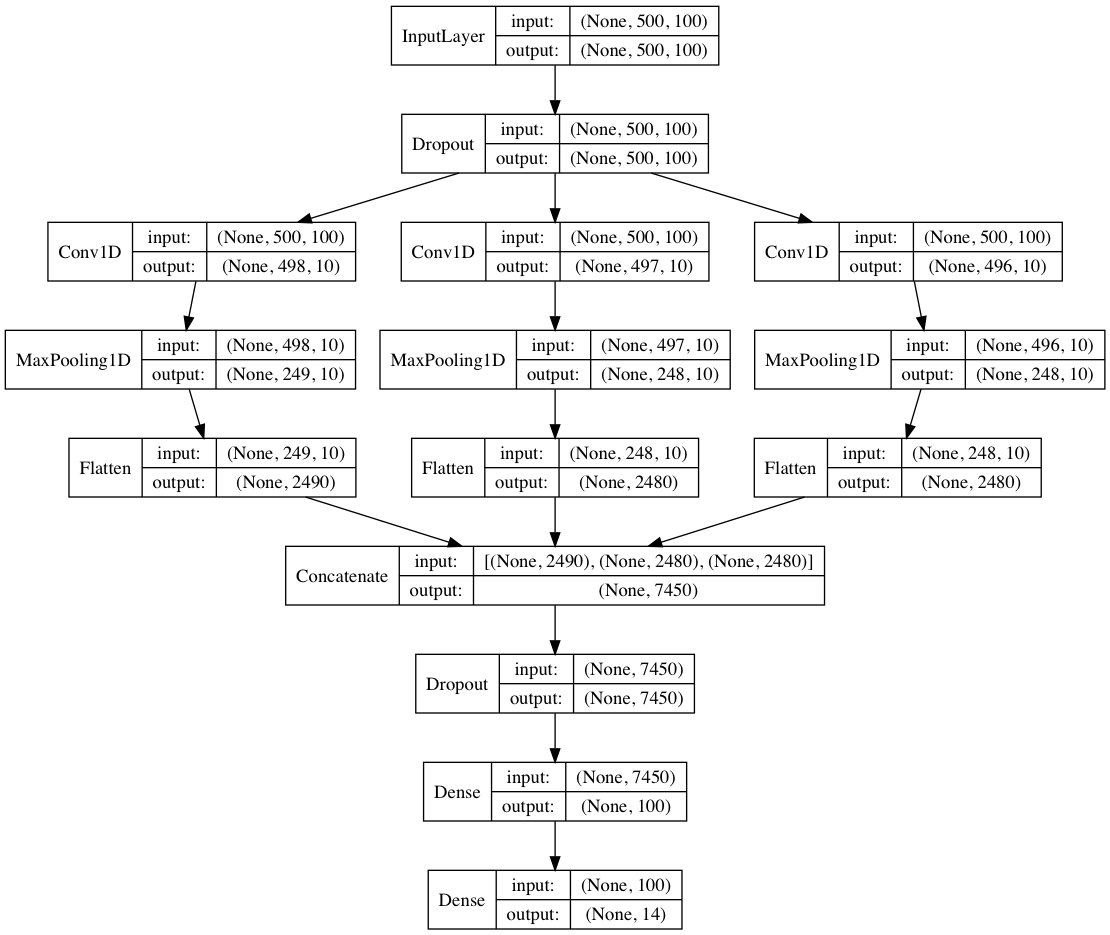
\includegraphics[height=0.35\textheight]{img/cnn}
	\caption{CNN with input consisting of $500$ words represented by $100$ dimensional GloVe vectors.}
	\label{fig:cnn}
\end{figure}

The best results are shown in \cref{tbl:cnn}.
\begin{table}[h!]
	\centering
	\begin{tabular}{|l|l|l|r|}\hline
		Document length & padding length & vector dim. & F1-macro score\\
		\hline
		$200$ chars   & 50 &  300 & $0.288$   \\
		$800$ chars   & 200 & 100 & $0.410$   \\
		$3200$ chars  & 500 & ? & $?$    \\
		\hline
	\end{tabular}
	\caption{Best performance for \textbf{CNN}.}
	\label{tbl:cnn}
\end{table}

\end{comment}

\textbf{TODO:} Put confusion matrix for each classifier and discuss.


